%%%%%%%%%%%%%%%%%%%%%%%%%%%%%%%%%%%%%%%%%%%%%%%%%%%%%%%%%%%%%%%%%%%%%%%%%%%%%%%%%%%%%%%%%%%%%%%%%%%%%%%%%%%%%%%%%%%%%%
\chapter{ Cosmological Background }\label{chap:marco}
%%%%%%%%%%%%%%%%%%%%%%%%%%%%%%%%%%%%%%%%%%%%%%%%%%%%%%%%%%%%%%%%%%%%%%%%%%%%%%%%%%%%%%%%%%%%%%%%%%%%%%%%%%%%%%%%%%%%%%

Cosmology is the branch of physics that studies the Universe as a whole, 
therefore, it attempts to explain its origin, evolution and the observed structure 
of the Universe,at least, at big scales. Hence, a coarse grained approximation is mandatory, 
this is, several approximations are necessary in the endeavour of such a task.

In this search, two major points are considered. The first one is the 
cosmological principle, it assumes that on sufficiently large scales the Universe can 
be considered homogeneous and isotropic. It can be understood homogeneity like invariance 
under traslation and isotropy like invariance under rotation. This principe stablishes that
the universe should appear the same for certain observers which are called fundamental observers,
i.e., observers located at each point for which the universe appears isotropic and
homogeneous. Then, there is no relative motion among them due to they are observing
the same structures. This finally allows to synchronize clocks defining an cosmic time. 

The overall isotropy and homogeneity have been observed, for example in the isotropy 
measured in the cosmic microwave background (CMB) radiation and the sponge like structure
of the distribution of galaxies. Until now, all observations have agreed with this asseveration.

\

The second point is that modern cosmology is based on general relativity, 
where Einstein field equations serve as a set of fundamental equations to
study the Universe at big scales, fortunately isotropy and homogeneity 
leds to a simple form of these.
From them, Friedmman equations provide a theoretical 
framework for the universe expansion, i.e., how the universe 
scale factor changes with
cosmic time.  Other important aspect is the global curvature that
depends on the universe total content of energy and matter and can only
take three possible values because of the cosmological principle. 

A standard model in cosmology is $\lambda$CDM, where additionally to an 
expanding universe, there is a dark energy component that accelerates 
its expansion. This is precisely the framework that is going to 
be used in this work. 

\

In this chapter, several basic concepts are going to be introduce to finally lead to 
bayronic acoustic oscillations (BAO). 

%&&&&&&&&&&&&&&&&&&&&&&&&&&&&&&&&&&&&&&&&&&&&&&&&&&&&&&&&&&&&&&&&&&&&&&&&&&&&&&&&&&&&&&&&&&&&&&&&&&&&&&&&&&&&&&&&&&&&&&
\section{ Robertson Walker Metric}
%&&&&&&&&&&&&&&&&&&&&&&&&&&&&&&&&&&&&&&&&&&&&&&&&&&&&&&&&&&&&&&&&&&&&&&&&&&&&&&&&&&&&&&&&&&&&&&&&&&&&&&&&&&&&&&&&&&&&&&

As was mentioned before, observations of the Universe at big scales show 
that it is homogenous and isotropic. This idea is also reinforced by the cosmic 
microwave background radiation (CMB), since it appears to have inhomogeneties
only at very small scales. Nevertheless, it can not be proven and it is taken
as a postulate. 

\begin{itemize}
\item Cosmological principle: \emph{ The Universe is homogeneous and isotropic 
at big scales.}

In this context, homogeneous is understood as the independence of the place 
where a reference system is defined, i.e., the structure of the Universe observed 
is the same no matter the reference system used. 
On the other hand, isotropy stablishes that regardless of the direction chosen, 
the same structure is going to be observed. Then, we are dealing with traslational
and rotational symmetry. 

These characteristics are observed on mega parsec scales, i.e., big scales. 
However, this is only valid for the actual epoch, the scale changes with time due 
to the expansion of the Universe. 


\item Weyl postulate :\emph{ Establishes that the geodesics, world lines of 
galaxies, do not intersect except in a singular point in a finite or infinite 
point, past.} 

This one defines a set of observers that move along the geodesics. 
The interception point allows to synchronize watches among different observers,
defining a cosmic time. Therefore, the distance between galaxies can
be measured at the same cosmic time. 

\end{itemize} 

There is another important fact to take into account before speaking of a metric,
the Universe is expanding. It was due to a research on near galaxies performed
by Edwin Hubble, that a redshift was found in most of the galaxies, i.e., they
are moving away from us. 
Considering this movement, one could conclude we are in the center of the 
expansion. But this conclusion is wrong, since the expansion Hubble law is
valid independently where the coordinate system is defined. 

\
A metric that satisfies homogenity and isotropy and additionally
contains a term that corresponds to the expansion is the 
Friedmann Lemaitre Robertson Walker metric. It is defined in 
general terms as $ds^2 = g_{\mu\nu}dx^{\mu}dx^{\nu}$, where $g_{\mu\nu}$
is the metric tensor and uses coordinates $x^{\alpha} = \{ct,x,y,z\}$.
The metric tensor takes the next form $ g_{\mu\nu} = diag\{1,-\frac{a^2}{1-k^2}
-a^2r^2,-a^2r^2\sin^2\theta\}$, and the metric is finally 

\begin{equation}
ds^2= c^2dt^2-a(t)^2\left[\frac{d^2r}{1-Kr^2} +r^2(d^2\theta
 + \sin^2\theta d^2\phi )\right]
\label{metric}
\end{equation} 	

The term $a(t)$ is the scale factor, it describes how the relative
distance between two fundamental observers changes with time. 
The term $K$ is the curvature constant for the actual time and defines
the Universe geometry. When $K=0$ an euclidean metric is recovered 
leading to a flat universe expanding indefinitly. If $K=1$ the Universe
would be described by a spherical geometry and it would collapse because
of its energy matter content. And finally, $K=-1$ corresponds to a
hyperbolic geometry where the Universe would be in accelerated expansion.  

One important aspect to consider is that the geometry depends on the 
total energy matter content, $\Omega_o$. This can be concluded from
te definition of the curvature constant $K = H_o^2(\Omega_o -1)/c^2$. 

Different cosmologies are shown in the figure \ref{factor}. 

%**********************************************************************************************************************
\begin{figure}[htbp]
       \centering
               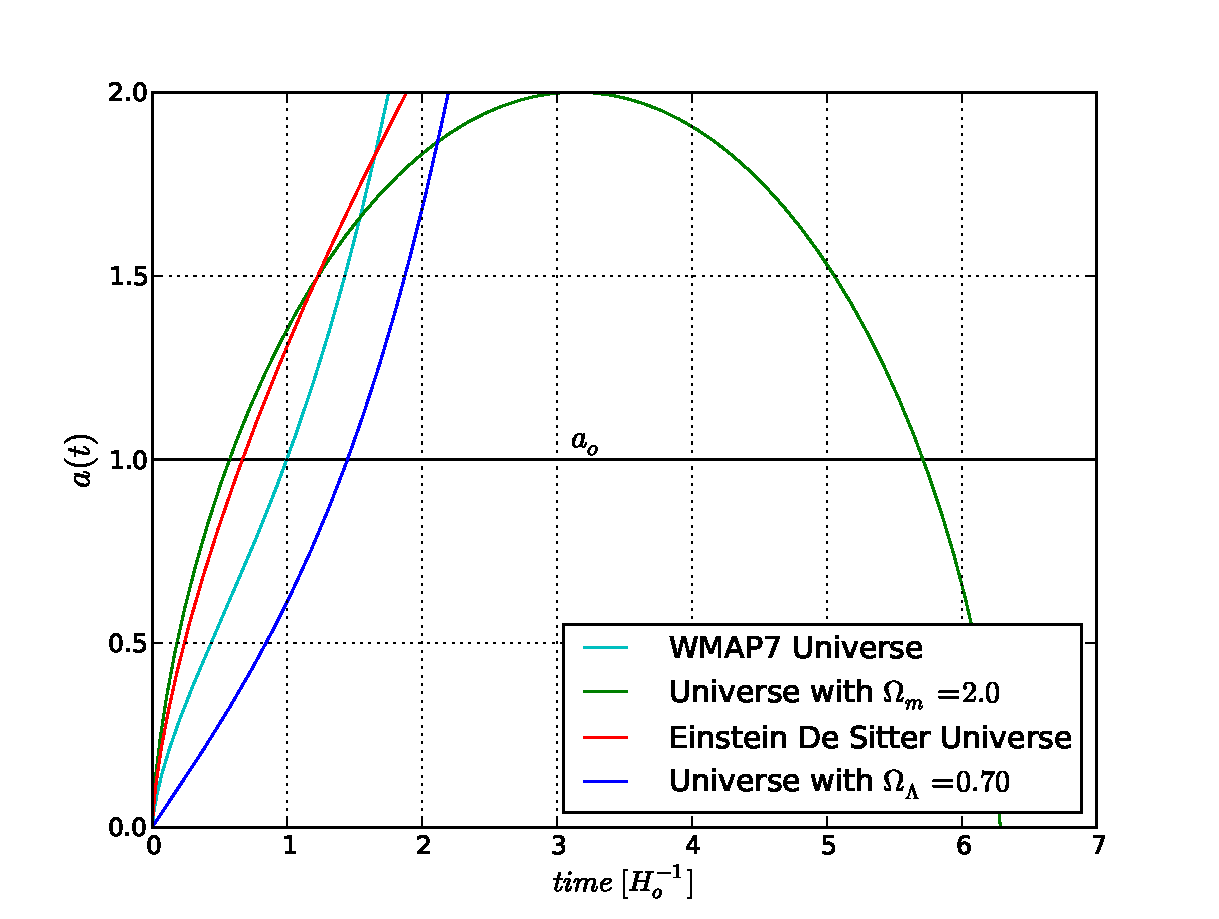
\includegraphics[width=0.8\textwidth]{Images/chapter2/factordeescala.pdf}
       \caption{ \small Scale factor as a time function. The Universe expansion for 
       different density contributions. A closed Universe is obtained when 
       $\Omega_m = \Omega_o>1$. Also, the WMAP7 parameters show an acelerated expansion. 
        }
       \label{factor}
 \end{figure}
%**********************************************************************************************************************

%&&&&&&&&&&&&&&&&&&&&&&&&&&&&&&&&&&&&&&&&&&&&&&&&&&&&&&&&&&&&&&&&&&&&&&&&&&&&&&&&&&&&&&&&&&&&&&&&&&&&&&&&&&&&&&&&&&&&&&
\section{Hilbert Einstein field equation}
%&&&&&&&&&&&&&&&&&&&&&&&&&&&&&&&&&&&&&&&&&&&&&&&&&&&&&&&&&&&&&&&&&&&&&&&&&&&&&&&&&&&&&&&&&&&&&&&&&&&&&&&&&&&&&&&&&&&&&&

At big scales, the most important fundamental interaction is the 
gravitational one. Hence, the theory of general relativity (TGR) is 
an essential tool in the study of the cosmos. 

At smaller scales, the Newtonian gravitational theory is valid, where, 
the Poisson equation offers a relation between the second derivative
of the field and the source of the field 

\[ \nabla^2\Phi=4\pi G\rho\]

this equation is obtained from TGR for low velocities and 
a weak gravitational field ($\Phi/c^2<< 1$). A key equation of TGR is
the Hilbert-Einstein field equation

\eq{
R_{\mu\nu}-\f{1}{2}g_{\mu\nu}R-g_{\mu\nu}\Lambda = \f{8\pi G}{c^4}T_{\mu\nu}
}

a 6 independent component tensorial equation. The first term of the left
is Ricci tensor (second derivatives of the metric tensor). The second one 
contains the scalar curvature that defines geometry. 
In the third term, $\Lambda$ is the cosmological constant, associated with
the vacuum density term and the accelerated expansion of the Universe.  

In the right side of the equation, the tensor energy-momentum is present.
It includes, as its name suggest, all the contributions to energy and momemtum. 

Hence, the left side of the equation has associated geometry terms, 
while the right one, the ones associated with the matter and energy distribution. 
Then, it could be assure geometry is determined by the matter-energy content 
of the Universe, though, strictly speaking, the energy-momentum tensor depends
in the metric tensor too. 

There is an interesting case of this tensor, when we are dealing with a perfect 
fluid, i.e., without viscosity, homogeneous and isotropic, such it can be expressed
as 

\[T^{\mu}_{\sigma}= diag\{c^2\rho,-P,-P,-P\}\]

where $\rho$ is the density and P is the fluid pressure. 
This shows that not only density causes curvature of space-time 
but also pressure. The Universe can be modelled with this particular
shape of the energy-momentum tensor. 


There are several solutions to the Einstein field equation but not
many in an analytical form, for example, Schwarzchild found the metric
of an estatic spherical mass. Other possible solution is the Kerr 
metric that corresponds to a rotating uncharged mass. The Robertson
Walker metric obviously satisfies these equations. 
	

%&&&&&&&&&&&&&&&&&&&&&&&&&&&&&&&&&&&&&&&&&&&&&&&&&&&&&&&&&&&&&&&&&&&&&&&&&&&&&&&&&&&&&&&&&&&&&&&&&&&&&&&&&&&&&&&&&&&&&&
\section{ Friedmann equations }
%&&&&&&&&&&&&&&&&&&&&&&&&&&&&&&&&&&&&&&&&&&&&&&&&&&&&&&&&&&&&&&&&&&&&&&&&&&&&&&&&&&&&&&&&&&&&&&&&&&&&&&&&&&&&&&&&&&&&&&


From HE field equations and the RW metric is posible to propose 
cosmological models that give account for the observed dynamics
in the Universe. In this direction, the components of the 
field equation can be taken, $\beta=\nu= 0$, time-time component,
and $ii=1,2,3$ (space-time components), from where

\begin{equation}
\frac{\ddot{a}}{a} = -\frac{4\pi G}{3 }\left( \rho + 3 \f{P}{c^2} \right)+\frac{\Lambda c^2}{3} 
\label{fried1}
\end{equation}

\[
\f{\ddot{a}}{a}+2\f{\dot{a}^2}{a^2}+2\f{c^2 K}{a^2} = 4\pi G\left( \rho-\frac{P}{c^2}\right)+\Lambda c^2
\]

\

here, it has been used the energy momentum tensor for an ideal fluid. 
The former expressions are the Friedmann equations and give account 
of Universe expansion dynamics. The terms involved are 
the scale factor $a(t)$ and it is equal to one for the actual epoch,
$a(t_o)=1$, also $\rho$ is the radiation and matter density, $P$ is
the total pressure.  

The equation \ref{fried1} has the form of force equation and it can
be parcially deduced from newtonian mechanic without the presion
and cosmological constant terms. A most convenient and used form
is obtained after algebraically manipulating them 


\begin{equation}
H(t)=\frac{\dot{a}^2}{a^2}=\frac{8 \pi G}{3}\left(\rho+\frac{\Lambda c^2}{8\pi G}\right) -\frac{Kc^2}{a^2}
\label{fried1}
\end{equation}

this one can be interpretated as an energy equation, where the first term in 
the right hand side is the potential energy. 
This equation also allows to define the Hubble parameter and for the 
actual epoch this coincides with the Hubble constant
$H(t_o)=H_o = 100h$ Km $s^{-1}$ $Mpc^{-1}$.

Aditionally \ref{fried2} can be expressed in terms of the critical
density, i.e.m the matter and energy amount neccesaries for the 
Universe to be flat. Therefore, if the Universe has a bigger density
it would collapse about itself.  Conversely, the Universe would
continue to expanding indefinitly. This quantity is defined as
$\rho_{crit}(t)= 3H(t)^2/8\pi G$.

Dividing \ref{fried2} by the Hubble constant $H_o$ and defining 
the density parameter  $\Omega_{i,o} = \rho_{i,o}/\rho_{crit}(t_o)$ 
with $i=m,r,\Lambda$ is obtained

\begin{equation}
\frac{H^2(z)}{H_o^{2}}=\Omega_{m,o}\left(1+z\right)^3+
\Omega_{r,o}\left(1+z\right)^4+ \Omega_{\Lambda,o} + ( 1-\Omega_o)
\left(1+z\right)
\label{fried2}
\end{equation}


where $\Omega_o=\Omega_{m,o} +\Omega_{r,o}+\Omega_{\Lambda,o}$. 
It has been introduced the relation between redshift and scale
factor $1+z=1/a$. The different contributions to the density 
to the Hubble parameters are observed, i.e., the matter, radiation
and vacuum density. Every component is a function of the 
Universe expansion, although the vacuum energy does not depend
on the redshift, this is, is constant through time. 

\

Initially the Universe was dominated by the radiation, during 
this epoch matter and radiation were coupled, i.e., the De Broglie 
electrons wavelenght were comparable to the radiation one. Because
of this, the photons free mean path is negligible causing the Universe
to be opaque. 

During this coupling, the radiation temperature is equal to the 
matter one and its behaviour is explained as a black body. 

As can be seen in the plot \ref{densidad}, from $z=3230$
matter becomes the major contribution the Universe density.
When $z=1100$ the temperature drop is big enough for the
recombination rate gets higher than the ionization one. 
Recombination refers to the formation of neutral atoms,
that was the ultimate cause to decoupling. 

The last radiation dispertion due to matter still can be
observed, and it is called cosmic radiation background (CMB).
Because of the Universe expansion, its temperature
has been droping, and it is nowadays around $T$ = $2.7K$. 
  
%**********************************************************************************************************************
\begin{figure}[htbp]
       \centering
               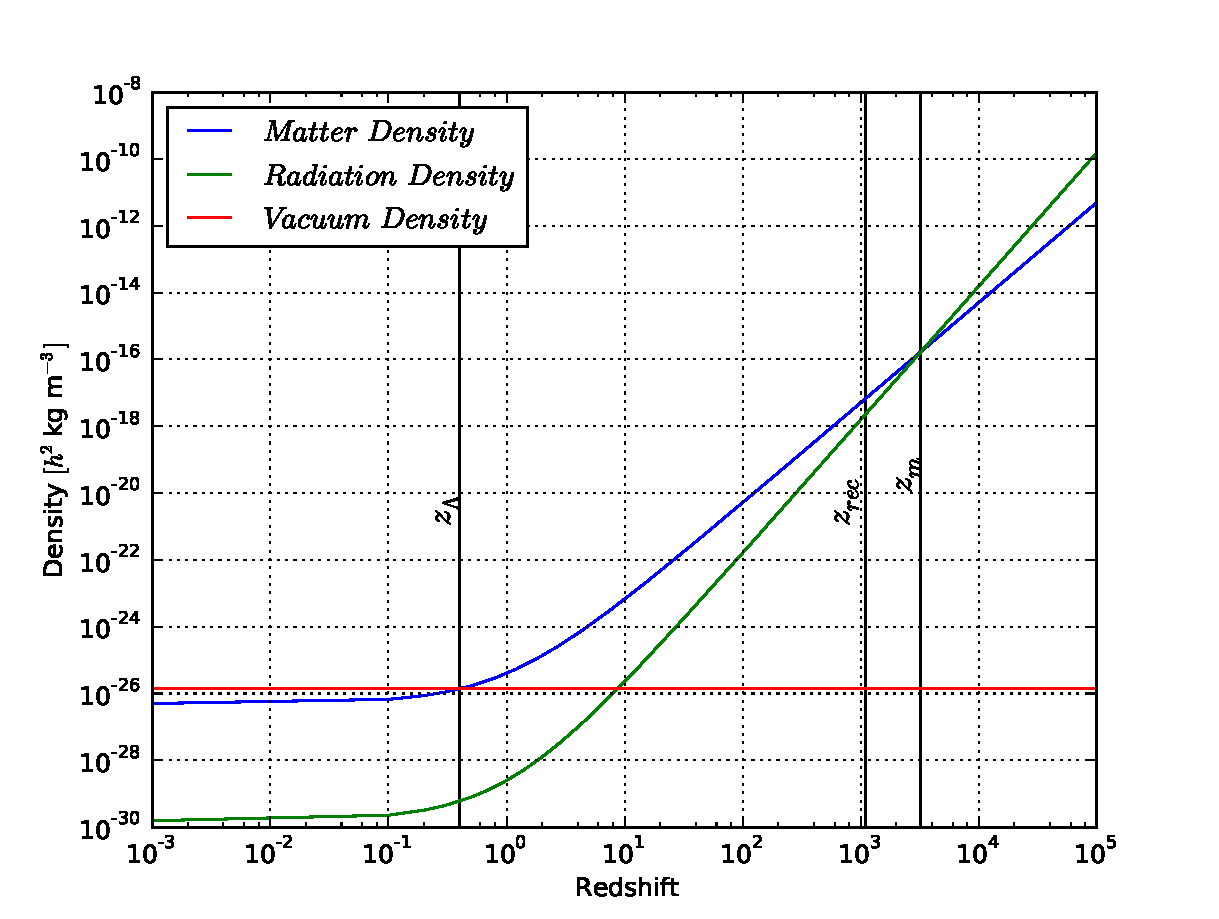
\includegraphics[width=0.8\textwidth]{Images/chapter2/density.pdf}
       \caption{ \small Dependence in redshift for $\Omega_\Lambda$, $\Omega_m$ and
       $\Omega_r$. The decoupling between matter and radiation is obtained when 
       $z_{rec}$.
        }
       \label{densidad}
 \end{figure}
%**********************************************************************************************************************

Nowadays, the dominant density component is vacuum, though it is a constant
since it does not depend on the scale factor $\rho_{\Lambda}=-c^4\Lambda/8\pi G$,
in contrast with matter, which depends on it as $a^{-3}$ and radiation as $a^{-4}$,
causing both components diminish in time. 

The cosmological constant is associated to a repulsive force, a opposed behaviour
to gravity, that could give into account the accelerated universe expansion. 

Therea are several solutions to \ref{fried2}, for instance in the Einstein de 
Sitter Universe, there are no radiation or vacuum contributions to the density
and the total density is $\Omega_o=1.0$ In this particular case, the solution
is

\[
t = \f{2}{3H_o}(1+z)^{-3/2}
\]

Therefore, depending on the chosen density values, the equation \ref{fried2}
has different solutions and one can expect several Universe models, i.e.,
depending on the parameters chost, the Universe evolution changes.  
In the case of WMAP9, the parameters used are shown in table\footnote{Table taken from \url{https://lambda.gsfc.nasa.gov/product/map/dr5/params/lcdm_wmap9.cfm}} \ref{WMAPtable}. 

\begin{table}
\begin{center}
  \begin{tabular}{ | c | c | c |}
    \hline \hline
    Parameter & Symbol & Best fit \\ \hline \hline 
    Hubble constant $(km/Mpc-s)$ & $H_0$ & 68.65$\pm$ 0.93 \\ \hline
    Baryon density & $\Omega_b h^2$ & 0.02248$\pm$0.00044 \\ \hline
    Cold dark matter density & $\Omega_c h^2$ & 0.1165$\pm$0.0024 \\  \hline
    Dark energy density & $\Omega_\Lambda$ & 0.705$\pm$0.0011\\ \hline
    Scalar spectral index & $n_s$ & 0.967$\pm$ 0.01 \\ \hline
    Sigma 8 & $\sigma_8$& 0.830 \\ \hline
  \end{tabular}
    \caption{ Fit cosmological parameters from WMAP+BAO nine-year results.}
  \label{WMAPtable}
\end{center}
\end{table}

Other possible Universe models are for example, one obtained when matter
density is the only contribution, and different total universe density.
If this former is bigger than one, the Universe obtained is closed. 
Other, it is one obtained when the universe is dominated for the vacuum
contribution. In this case, the Universe is always open. When all the 
contributions are present, the Universe can be open or closed depending on
total density paremeter.

%&&&&&&&&&&&&&&&&&&&&&&&&&&&&&&&&&&&&&&&&&&&&&&&&&&&&&&&&&&&&&&&&&&&&&&&&&&&&&&&&&&&&&&&&&&&&&&&&&&&&&&&&&&&&&&&&&&&&&&
\section{ State equation }
%&&&&&&&&&&&&&&&&&&&&&&&&&&&&&&&&&&&&&&&&&&&&&&&&&&&&&&&&&&&&&&&&&&&&&&&&&&&&&&&&&&&&&&&&&&&&&&&&&&&&&&&&&&&&&&&&&&&&&&




%&&&&&&&&&&&&&&&&&&&&&&&&&&&&&&&&&&&&&&&&&&&&&&&&&&&&&&&&&&&&&&&&&&&&&&&&&&&&&&&&&&&&&&&&&&&&&&&&&&&&&&&&&&&&&&&&&&&&&&
\section{ Perturbation evolution in the newtonian regimen }
%&&&&&&&&&&&&&&&&&&&&&&&&&&&&&&&&&&&&&&&&&&&&&&&&&&&&&&&&&&&&&&&&&&&&&&&&&&&&&&&&&&&&&&&&&&&&&&&&&&&&&&&&&&&&&&&&&&&&&&

%######################################################################################################################
\subsection{ Newtonian description  }
%######################################################################################################################
%######################################################################################################################
\subsection{ Jeans Inestability}
%######################################################################################################################



%&&&&&&&&&&&&&&&&&&&&&&&&&&&&&&&&&&&&&&&&&&&&&&&&&&&&&&&&&&&&&&&&&&&&&&&&&&&&&&&&&&&&&&&&&&&&&&&&&&&&&&&&&&&&&&&&&&&&&&
\section{ Statistical properties of cosmological perturbations }
%&&&&&&&&&&&&&&&&&&&&&&&&&&&&&&&&&&&&&&&&&&&&&&&&&&&&&&&&&&&&&&&&&&&&&&&&&&&&&&&&&&&&&&&&&&&&&&&&&&&&&&&&&&&&&&&&&&&&&&
%######################################################################################################################
\subsection{ Gaussian Random fields }
%######################################################################################################################
%######################################################################################################################
\subsection{ Linear perturbation spectrum }
%######################################################################################################################
%-----------------------------------------------------------------------------------------------------------
\subsubsection{ Initial power spectrum }
%-----------------------------------------------------------------------------------------------------------
%-----------------------------------------------------------------------------------------------------------
\subsubsection{ Amplitude of the linear power spectrum }
%-----------------------------------------------------------------------------------------------------------
%-----------------------------------------------------------------------------------------------------------
\subsubsection{ Standard deviation }
%-----------------------------------------------------------------------------------------------------------



%&&&&&&&&&&&&&&&&&&&&&&&&&&&&&&&&&&&&&&&&&&&&&&&&&&&&&&&&&&&&&&&&&&&&&&&&&&&&&&&&&&&&&&&&&&&&&&&&&&&&&&&&&&&&&&&&&&&&&&
\section{ Higher order perturbation theory }
%&&&&&&&&&&&&&&&&&&&&&&&&&&&&&&&&&&&&&&&&&&&&&&&&&&&&&&&&&&&&&&&&&&&&&&&&&&&&&&&&&&&&&&&&&&&&&&&&&&&&&&&&&&&&&&&&&&&&&&
%######################################################################################################################
\subsection{ Zeldovich approximation }
%######################################################################################################################


%&&&&&&&&&&&&&&&&&&&&&&&&&&&&&&&&&&&&&&&&&&&&&&&&&&&&&&&&&&&&&&&&&&&&&&&&&&&&&&&&&&&&&&&&&&&&&&&&&&&&&&&&&&&&&&&&&&&&&&
\section{ Cosmic density field }
%&&&&&&&&&&&&&&&&&&&&&&&&&&&&&&&&&&&&&&&&&&&&&&&&&&&&&&&&&&&&&&&&&&&&&&&&&&&&&&&&&&&&&&&&&&&&&&&&&&&&&&&&&&&&&&&&&&&&&&
%######################################################################################################################
\subsection{ Correlation functions }
%######################################################################################################################
%######################################################################################################################
\subsection{ Mass moments }
%######################################################################################################################
%######################################################################################################################
\subsection{ Clustering in the real and redshift space }
%######################################################################################################################
%-----------------------------------------------------------------------------------------------------------
\subsubsection{ Redshift distortions }
%-----------------------------------------------------------------------------------------------------------
%-----------------------------------------------------------------------------------------------------------
\subsubsection{ Real space correlation functions }
%-----------------------------------------------------------------------------------------------------------

%&&&&&&&&&&&&&&&&&&&&&&&&&&&&&&&&&&&&&&&&&&&&&&&&&&&&&&&&&&&&&&&&&&&&&&&&&&&&&&&&&&&&&&&&&&&&&&&&&&&&&&&&&&&&&&&&&&&&&&
\section{ Baryonic acoustic oscillations }
%&&&&&&&&&&&&&&&&&&&&&&&&&&&&&&&&&&&&&&&&&&&&&&&&&&&&&&&&&&&&&&&&&&&&&&&&&&&&&&&&&&&&&&&&&&&&&&&&&&&&&&&&&&&&&&&&&&&&&&
